\subsection{Representative Fits}
  \label{subsec:fits}

  We illustrate the performance of the effective model on representative
  galaxies spanning different surface-density regimes.
  The goal is not to emphasize isolated best cases, but to show typical
  behaviors observed across the full SPARC sample.

  High-surface-density galaxies are well described by Newtonian dynamics in
  their inner regions.
  Deviations from Newtonian predictions appear only at large radii, where the
  baryonic acceleration drops below the saturation scale.
  The resulting rotation curves flatten smoothly, without requiring extended
  mass halos, in agreement with observed trends across high-surface-brightness
  disks~\cite{Lelli2016SPARC}.

  Low-surface-brightness galaxies probe the saturated regime over most of their
  radial extent.
  In these systems, the effective acceleration departs from Newtonian behavior
  already at small radii, naturally producing slowly rising and asymptotically
  flat rotation curves, a feature commonly observed in diffuse systems~\cite{McGaugh2016}.

  Across the sample, the model reproduces the observed diversity of rotation
  curve shapes.
  This diversity arises solely from differences in the baryonic mass
  distribution and surface density, not from variations in the effective
  parameters.

  The galaxies shown in Fig.~\ref{fig:rotation-curves} are selected as
  representative well-fitted systems spanning rising, nearly flat,
  and slowly declining rotation curves.
  The saturation scale $a_\star$ is fixed globally from the full-sample
  analysis discussed in Section~\ref{subsec:universality}.
  No galaxy-dependent adjustment of $a_\star$ is performed.

  \begin{figure}
    \centering
    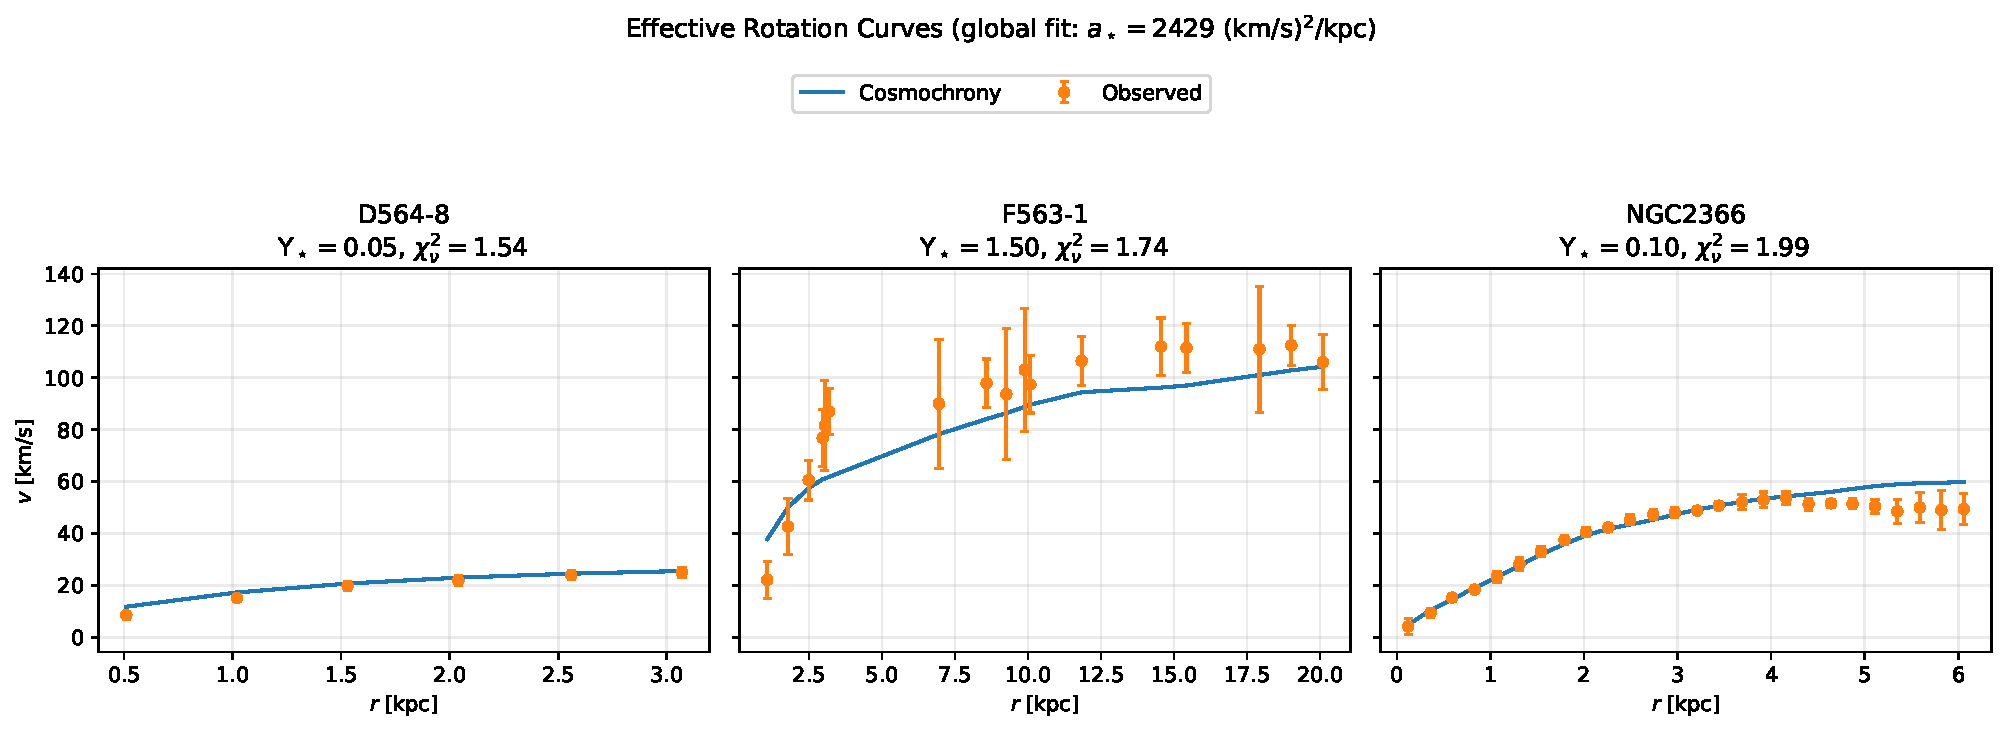
\includegraphics[width=\linewidth]{../code/03-rotation_curves/galaxy_rotcurves_showcase}
    \caption[Representative SPARC rotation curves]{
      Representative galaxy rotation curves from the SPARC sample.
      Observed circular velocities (points) are compared with the effective model
      prediction (solid lines) computed from the baryonic mass distribution alone.
      The three systems span distinct surface-density regimes and kinematic
      behaviors (rising, nearly flat, and mildly declining).
      A single universal saturation scale $a_\star$, determined from the full
      sample, is used for all galaxies.
      The only galaxy-dependent parameter is the stellar mass-to-light ratio
      $\Upsilon_\star$, fitted within a physically motivated interval.
      The code used to generate these curves is publicly available
      \protect\cite{CosmochronySimulation}.
    }
    \label{fig:rotation-curves}
  \end{figure}

  Representative examples illustrating these behaviors are shown in
  Fig.~\ref{fig:rotation-curves}.
